% Intended LaTeX compiler: pdflatex
\documentclass[letterpaper]{article}
\usepackage[utf8]{inputenc}
\usepackage[T1]{fontenc}
\usepackage{graphicx}
\usepackage{longtable}
\usepackage{wrapfig}
\usepackage{rotating}
\usepackage[normalem]{ulem}
\usepackage{amsmath}
\usepackage{amssymb}
\usepackage{capt-of}
\usepackage{hyperref}
\usepackage{lmodern} % Ensures we have the right font
\usepackage{listings} % Syntax highlighting
\usepackage{lmodern} % Ensures we have the right font
\usepackage[utf8]{inputenc}
\usepackage{graphicx}
\usepackage{amsmath, amsthm, amssymb}
\usepackage[table, xcdraw]{xcolor}
\date{}
\title{Resultados}
\hypersetup{
 pdfauthor={Oriol Julián},
 pdftitle={Resultados},
 pdfkeywords={},
 pdfsubject={},
 pdfcreator={Emacs 28.2 (Org mode 9.5.5)}, 
 pdflang={Spanish}}
\begin{document}

\maketitle
\tableofcontents


\section{Notación}
\label{sec:org971a5b9}
\textbf{fun} = Mínimo local hallado de la función \emph{execute\textunderscore circuit} con el optimizador
\newline
\textbf{p} = Número de capas (a mayor número el circuito es más profundo)
\newline
\textbf{theta} = Lista de parámetros [\(\beta\)\textsubscript{1}, \ldots{}, \(\beta\)\textsubscript{p}, \(\gamma\)\textsubscript{1}, \ldots{}, \(\gamma\)\textsubscript{p}] del circuito cuántico
\newline
\textbf{num iterations} = Número de iteraciones del compilador necesarias para hallar el mínimo
\newline
\textbf{seed\textunderscore simulator} = Semilla utilizada en la ejecución del circuito para fijar la aleatoriedad en \emph{backend.run()}
\newline
\textbf{X\textsubscript{ij}} = Se refiere a la arista \textbf{i} -> \textbf{j}. 1 Si dicha arista es parte del camino resultante, 0 en otro caso
\newline
\textbf{q\textsubscript{n}} = Qubit enésimo
\newline
q\textsubscript{4}q\textsubscript{3}q\textsubscript{2}q\textsubscript{1}q\textsubscript{0} = X\textsubscript{23}X\textsubscript{13}X\textsubscript{12}X\textsubscript{02}X\textsubscript{01}
\newpage

\section{Primer grafo sin restricción}
\label{sec:org10bc7e9}
\begin{center}
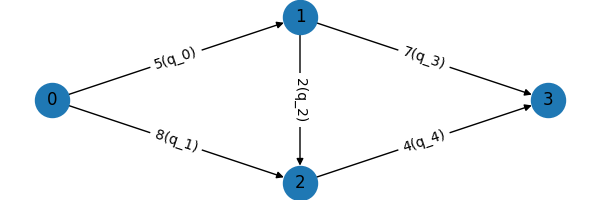
\includegraphics[width=.9\linewidth]{./img/primer_grafo/primer_grafo.png}
\end{center}
\newpage
\subsection{Aer - Versión del paper (primer\textunderscore grafo/aer-qaoa.ipynb)}
\label{sec:orgbd8f06a}
Pruebas realizadas sobre la versión del código sin la restricción\newline
    \textbf{X\textsubscript{13} + X\textsubscript{23} = 1}\newline

Versión equivalente a la de [\href{https://www.mdpi.com/1424-8220/22/19/7570/xml}{Multi-Objective Routing Optimization for 6G Communication Networks Using a Quantum Approximate Optimization Algorithm-sensors-22-07570-v2}]

\begin{itemize}
\item \textbf{Estadísticas:}

Realizando la ejecución 1000 veces se han obtenido como caminos resultantes los siguientes:

\begin{center}
\begin{tabular}{|r|l|r|}
\hline
\textbf{Qubits} & \textbf{Camino} & \textbf{Frecuencia} (1000)\\
\hline
10101 & X\textsubscript{01}X\textsubscript{12}X\textsubscript{23} & 917\\
10110 & X\textsubscript{02}X\textsubscript{12}X\textsubscript{23} & 82\\
01001 & X\textsubscript{01}X\textsubscript{13} & 1\\
\hline
\end{tabular}
\end{center}
\end{itemize}
\newpage

\subsubsection{Caso correcto}
\label{sec:orgdce2d85}

\begin{center}
\begin{tabular}{|r|l|r|r|}
\hline
\textbf{fun} & \textbf{theta} & \textbf{num iterations} & \textbf{seed\textunderscore simulator}\\
\hline
29.63 & [0.7739, 0.9302] & 29 & 10\\
\hline
\end{tabular}
\end{center}

\begin{figure}[htbp]
\centering
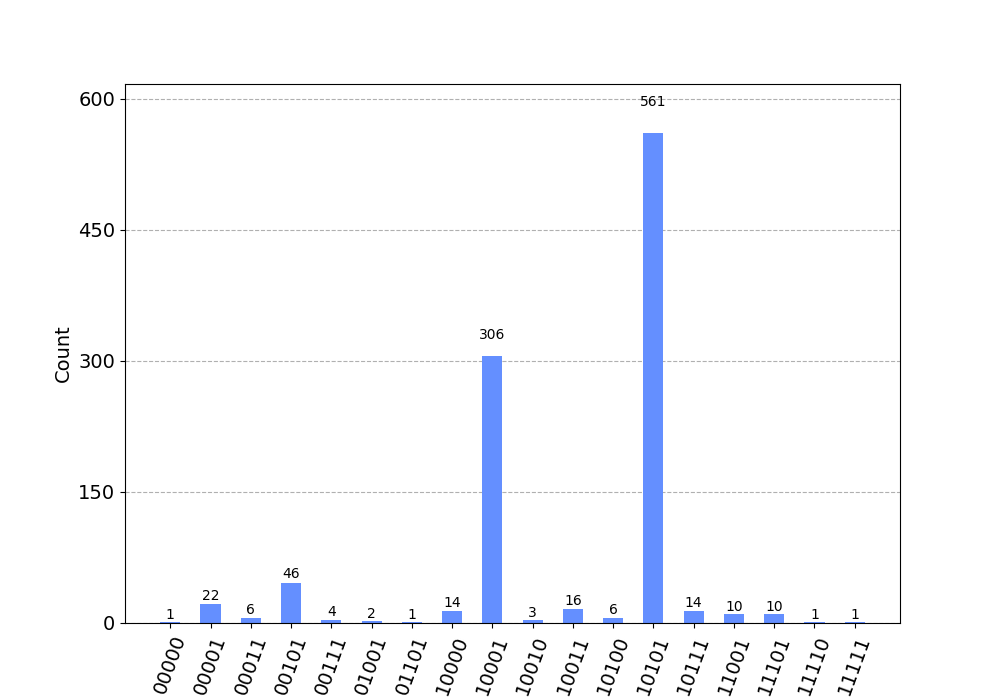
\includegraphics[scale=0.5]{./img/primer_grafo/sin_restriccion_extra/primer_paper_aer_correcto.png}
\caption{seed\textunderscore simulator=10}
\end{figure}

Mejor resultado: 10101 (q\textsubscript{4}q\textsubscript{3}q\textsubscript{2}q\textsubscript{1}q\textsubscript{0} = X\textsubscript{23}X\textsubscript{13}X\textsubscript{12}X\textsubscript{02}X\textsubscript{01})

Camino: X\textsubscript{01}X\textsubscript{12}X\textsubscript{23} (Camino óptimo)

\newpage

\subsubsection{Caso erróneo}
\label{sec:orgf8d62c5}

\begin{center}
\begin{tabular}{|r|l|r|r|}
\hline
\textbf{fun} & \textbf{theta} & \textbf{num iterations} & \textbf{seed\textunderscore simulator}\\
\hline
52.79 & [0.6320  0.7177] & 35 & 21\\
\hline
\end{tabular}
\end{center}

\begin{figure}[htbp]
\centering
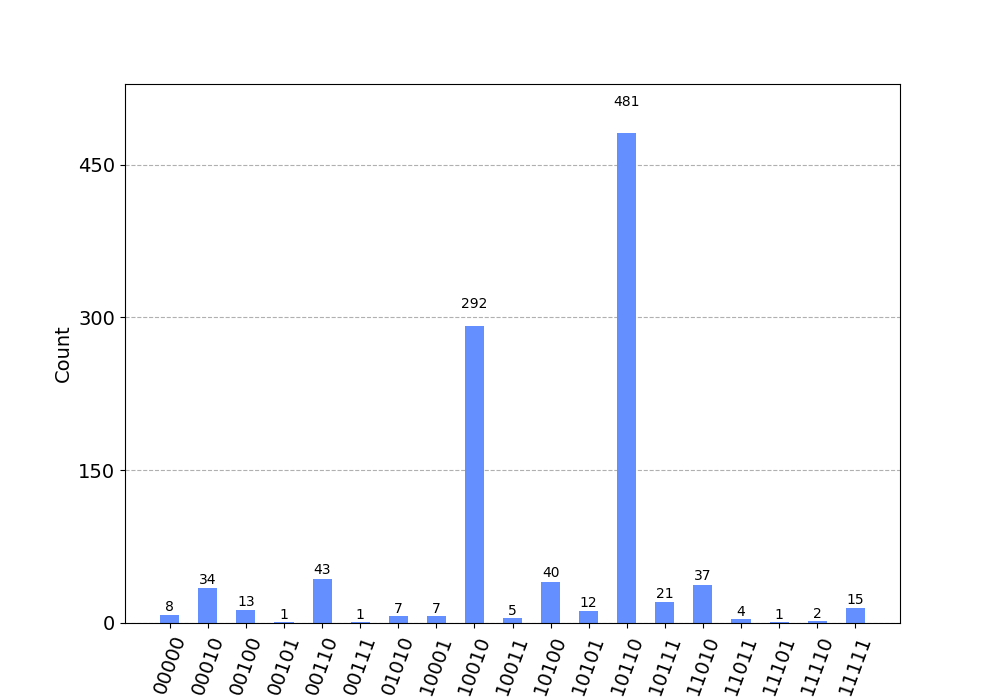
\includegraphics[scale=0.5]{./img/primer_grafo/sin_restriccion_extra/primer_paper_aer_erroneo.png}
\caption{seed\textunderscore simulator=21}
\end{figure}

Mejor resultado: 10110 (q\textsubscript{4}q\textsubscript{3}q\textsubscript{2}q\textsubscript{1}q\textsubscript{0} = X\textsubscript{23}X\textsubscript{13}X\textsubscript{12}X\textsubscript{02}X\textsubscript{01})

Camino: X\textsubscript{02}X\textsubscript{12}X\textsubscript{23} (Camino incorrecto. Rompe 2 restricciones)

Restricciones rotas: \newline
    \textbf{X\textsubscript{02}+X\textsubscript{12}=X\textsubscript{23}} \newline
    \textbf{X\textsubscript{01}=X\textsubscript{12}+X\textsubscript{13}} \newline

\newpage

\subsubsection{Caso subóptimo}
\label{sec:orgcbe93dc}

Obtenido a mano (no se ha encontrado ninguna semilla que diese este resultado)

\begin{center}
\begin{tabular}{|r|l|}
\hline
\textbf{fun} & \textbf{theta}\\
\hline
67.33 & [-0.4811, 1.566]\\
\hline
\end{tabular}
\end{center}

\begin{center}
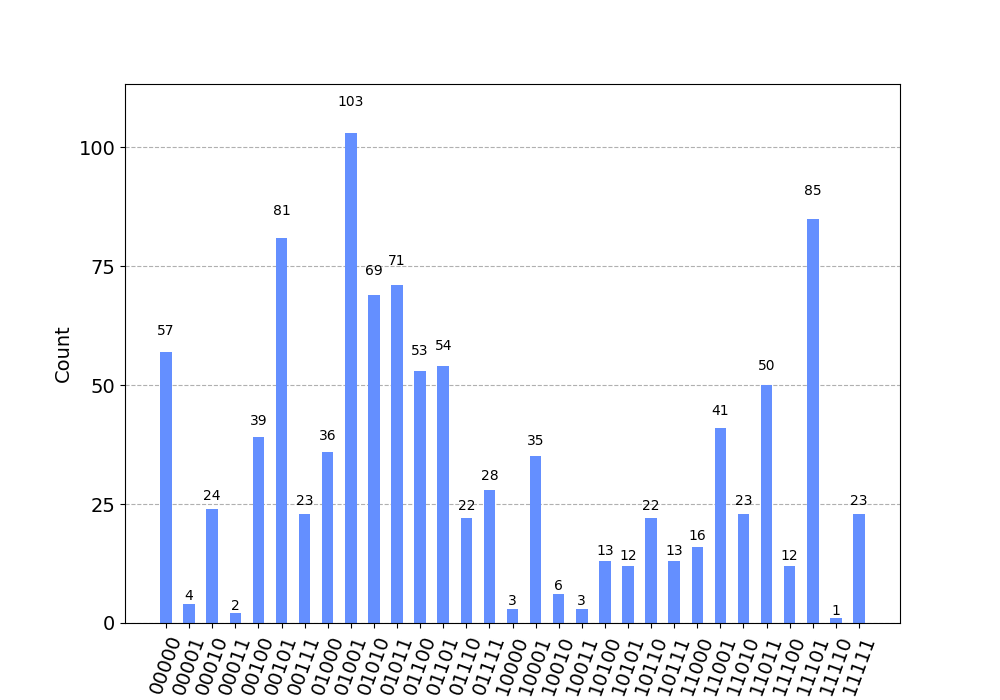
\includegraphics[scale=0.5]{./img/primer_grafo/sin_restriccion_extra/primer_paper_aer_suboptimo.png}
\end{center}

Mejor resultado: 01001 (q\textsubscript{4}q\textsubscript{3}q\textsubscript{2}q\textsubscript{1}q\textsubscript{0} = X\textsubscript{23}X\textsubscript{13}X\textsubscript{12}X\textsubscript{02}X\textsubscript{01})

Camino: X\textsubscript{01}X\textsubscript{13} (Camino subóptimo, pero no se rompe ninguna restricción)

\newpage

\subsubsection{Utilizando el parámetro \textbf{theta} obtenido en el artículo}
\label{sec:org7f6b227}

\begin{center}
\begin{tabular}{|r|l|}
\hline
\textbf{fun} & \textbf{theta}\\
\hline
65.40 & [0.28517317, -5.05969577]\\
\hline
\end{tabular}
\end{center}

\begin{center}
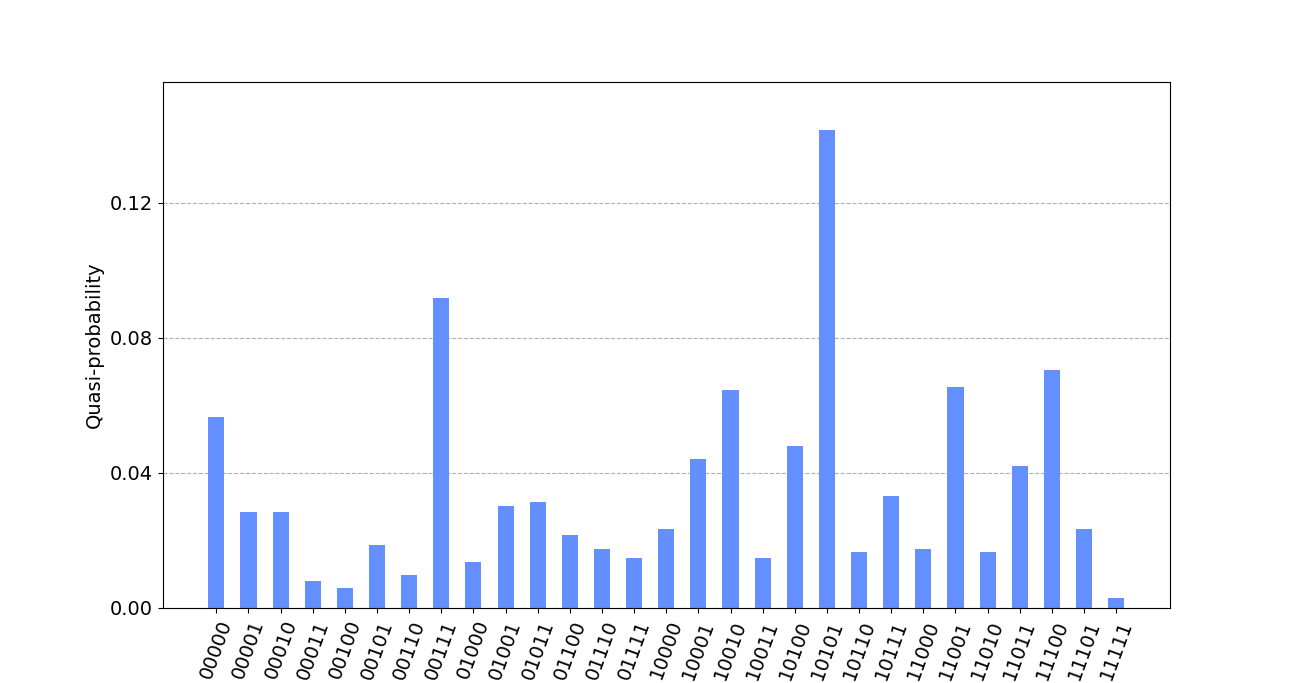
\includegraphics[scale=0.5]{./img/primer_grafo/sin_restriccion_extra/primer_paper_aer_resultado.png}
\end{center}

Mejor resultado: 10101 (q\textsubscript{4}q\textsubscript{3}q\textsubscript{2}q\textsubscript{1}q\textsubscript{0} = X\textsubscript{23}X\textsubscript{13}X\textsubscript{12}X\textsubscript{02}X\textsubscript{01})

Camino: X\textsubscript{01}X\textsubscript{12}X\textsubscript{23} (Camino óptimo)

La gráfica resultante es muy similar a la versión que se intenta replicar. \textbf{fun} tiene resultados muy altos, entre 65 y 70 (en comparación con la versión del código con la restricción extra).

\newpage

\subsubsection{Rz(*2), Rzz(*2), Rx(*2)}
\label{sec:org67d58bc}
\lstset{language=Python,label= ,caption= ,captionpos=b,numbers=none}
\begin{lstlisting}
circuit.rz(coef * 2, q_idx)
circuit.rzz(coef * gamma[p] * 2, q_idxs[0], q_idxs[1])
circuit.rx(beta[p] * 4, q_idx)
\end{lstlisting}

\begin{center}
\begin{tabular}{|r|l|r|}
\hline
\textbf{Qubits} & \textbf{Camino} & \textbf{Frecuencia (1000)}\\
\hline
11010 & X\textsubscript{02}X\textsubscript{13}X\textsubscript{23} & 845\\
11001 &  & 88\\
01010 &  & 5\\
11011 &  & 14\\
00101 &  & 21\\
00010 &  & 1\\
10110 &  & 14\\
10101 &  & 3\\
01001 &  & 5\\
10010 &  & 2\\
00110 &  & 2\\
\hline
\end{tabular}
\end{center}

\subsubsection{coef *= 2}
\label{sec:org509f86f}
\lstset{language=Python,label= ,caption= ,captionpos=b,numbers=none}
\begin{lstlisting}
circuit.rz(2 * coef, q_idx)
circuit.rzz(2 * coef * gamma[p], q_idxs[0], q_idxs[1])
circuit.rx(beta[p] * 2, q_idx)
\end{lstlisting}

\begin{center}
\begin{tabular}{|r|l|r|}
\hline
\textbf{Qubits} & \textbf{Camino} & \textbf{Frecuencia (1000)}\\
\hline
11010 & X\textsubscript{02}X\textsubscript{13}X\textsubscript{23} & 966\\
11101 &  & 2\\
00101 &  & 18\\
01010 &  & 8\\
11001 &  & 3\\
00110 &  & 1\\
10110 &  & 2\\
\hline
\end{tabular}
\end{center}

Da un mismo error un porcentaje de veces muy alto. Error muy fiable.

\subsubsection{Coef /= 2}
\label{sec:orgabb8c99}
\lstset{language=Python,label= ,caption= ,captionpos=b,numbers=none}
\begin{lstlisting}
circuit.rz(1/2 * coef, q_idx)
circuit.rzz(1/2 * coef * gamma[p], q_idxs[0], q_idxs[1])
circuit.rx(beta[p] * 2, q_idx)
\end{lstlisting}

\begin{center}
\begin{tabular}{|r|l|r|}
\hline
\textbf{Qubits} & \textbf{Camino} & \textbf{Frecuencia (1000)}\\
\hline
00000 &  & 1000\\
\hline
\end{tabular}
\end{center}

\newpage

\subsubsection{\(\beta\) /= 2}
\label{sec:org4e7b0ec}
\lstset{language=Python,label= ,caption= ,captionpos=b,numbers=none}
\begin{lstlisting}
circuit.rz(coef, q_idx)
circuit.rzz(coef * gamma[p], q_idxs[0], q_idxs[1])
circuit.rx(beta[p], q_idx)
\end{lstlisting}

\begin{center}
\begin{tabular}{|r|l|r|}
\hline
\textbf{Qubits} & \textbf{Camino} & \textbf{Frecuencia (1000)}\\
\hline
10101 & \uline{Óptimo} & 986\\
10110 &  & 14\\
\hline
\end{tabular}
\end{center}

\begin{figure}[htbp]
\centering
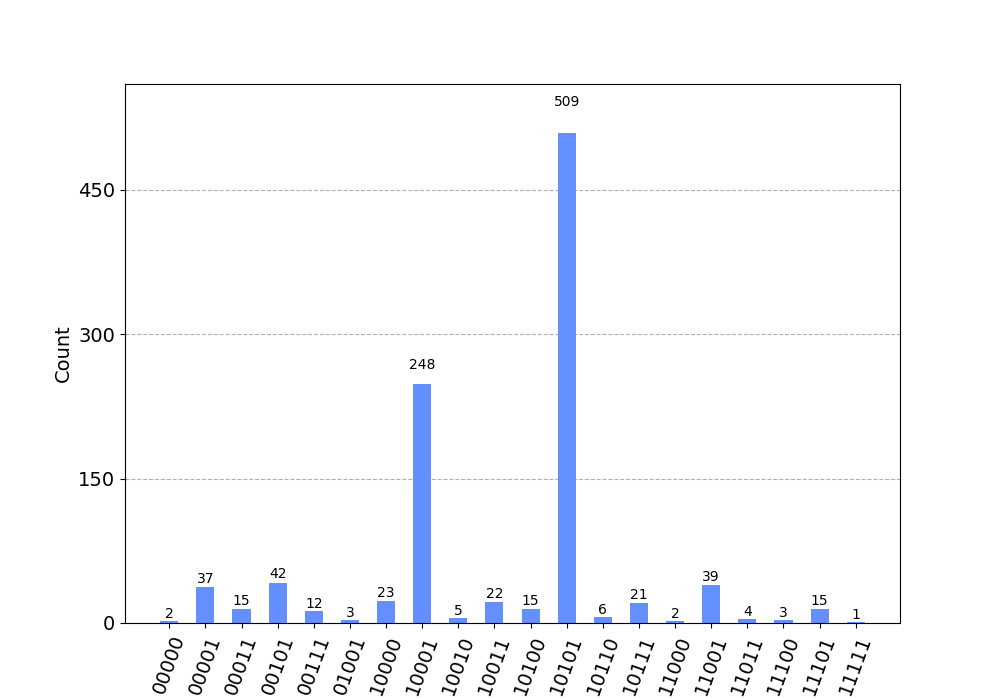
\includegraphics[scale=0.5]{./img/primer_grafo/sin_restriccion_extra/primer_paper_aer_beta-div-2.png}
\caption{Mejor resultado}
\end{figure}

\newpage

\subsubsection{\(\gamma\) /= 2}
\label{sec:org1fc1f33}
\lstset{language=Python,label= ,caption= ,captionpos=b,numbers=none}
\begin{lstlisting}
circuit.rz(coef, q_idx)
circuit.rzz(coef * gamma[p] / 2, q_idxs[0], q_idxs[1])
circuit.rx(beta[p] * 2, q_idx)
\end{lstlisting}

\begin{center}
\begin{tabular}{|r|l|r|}
\hline
\textbf{Qubits} & \textbf{Camino} & \textbf{Frecuencia (1000)}\\
\hline
10101 & \uline{Óptimo} & 1000\\
\hline
\end{tabular}
\end{center}

\newpage

\subsubsection{\(\beta\) /= 2, \(\gamma\) /= 2}
\label{sec:org63bfb7b}
\lstset{language=Python,label= ,caption= ,captionpos=b,numbers=none}
\begin{lstlisting}
circuit.rz(coef, q_idx)
circuit.rzz(coef * gamma[p] / 2, q_idxs[0], q_idxs[1])
circuit.rx(beta[p], q_idx)
\end{lstlisting}


\begin{itemize}
\item num layers = 1:
\begin{center}
\begin{tabular}{|r|l|r|}
\hline
\textbf{Qubits} & \textbf{Camino} & \textbf{Frecuencia (1000)}\\
\hline
10101 & \uline{Óptimo} & 1000\\
\hline
\end{tabular}
\end{center}

\item num layers = 2:
\begin{center}
\begin{tabular}{|r|l|r|}
\hline
\textbf{Qubits} & \textbf{Camino} & \textbf{Frecuencia (1000)}\\
\hline
10101 &  & 960\\
10001 &  & 28\\
11001 &  & 12\\
\hline
\end{tabular}
\end{center}

\item num layers = 3:
\begin{center}
\begin{tabular}{|r|l|r|}
\hline
\textbf{Qubits} & \textbf{Camino} & \textbf{Frecuencia (1000)}\\
\hline
10101 &  & 565\\
10001 &  & 111\\
11101 &  & 87\\
\ldots{} &  & \ldots{}\\
\hline
\end{tabular}
\end{center}
\end{itemize}

\newpage

\subsubsection{\(\beta\)\textsubscript{0} = 0.5, \(\gamma\)\textsubscript{0} = 0.5}
\label{sec:org1201cfd}

\begin{itemize}
\item num layers = 1:
\begin{center}
\begin{tabular}{|r|l|r|}
\hline
\textbf{Qubits} & \textbf{Camino} & \textbf{Frecuencia (1000)}\\
\hline
10101 &  & 1000\\
\hline
\end{tabular}
\end{center}

\item num layers = 2:
\begin{center}
\begin{tabular}{|r|l|r|}
\hline
\textbf{Qubits} & \textbf{Camino} & \textbf{Frecuencia (1000)}\\
\hline
10101 &  & 992\\
11001 &  & 8\\
\hline
\end{tabular}
\end{center}

\item num layers = 3:
\begin{center}
\begin{tabular}{|r|l|r|}
\hline
\textbf{Qubits} & \textbf{Camino} & \textbf{Frecuencia (1000)}\\
\hline
10101 &  & 469\\
11101 &  & 198\\
11011 &  & 88\\
\ldots{} &  & \ldots{}\\
\hline
\end{tabular}
\end{center}
\end{itemize}

\newpage

\subsubsection{Original pero variar num layers}
\label{sec:org1869737}

Al aumentar el número de capas se obtienen resultados mucho peores (tal vez esté mal implementado)
\begin{itemize}
\item num layers = 1: (Igual que tabla de estadisticas normal)
\begin{center}
\begin{tabular}{|r|l|r|}
\hline
\textbf{Qubits} & \textbf{Camino} & \textbf{Frecuencia (1000)}\\
\hline
10101 &  & 913\\
10110 &  & 86\\
01001 &  & 1\\
\hline
\end{tabular}
\end{center}

\item num layers = 2:
\begin{center}
\begin{tabular}{|r|l|r|}
\hline
\textbf{Qubits} & \textbf{Camino} & \textbf{Frecuencia (1000)}\\
\hline
10101 &  & 646\\
10010 &  & 75\\
10110 &  & 70\\
10001 &  & 49\\
\ldots{} &  & \ldots{}\\
\hline
\end{tabular}
\end{center}

\item num layers = 3:
\begin{center}
\begin{tabular}{|r|l|r|}
\hline
\textbf{Qubits} & \textbf{Camino} & \textbf{Frecuencia (1000)}\\
\hline
10101 &  & 634\\
10010 &  & 92\\
10001 &  & 84\\
01001 &  & 66\\
00000 &  & 36\\
\hline
\end{tabular}
\end{center}
\end{itemize}
\newpage
\subsection{Aer simulator sin restricción extra y P = 40}
\label{sec:org6522d62}
\subsubsection{Modificadores paper}
\label{sec:org4d38c7d}
\lstset{language=Python,label= ,caption= ,captionpos=b,numbers=none}
\begin{lstlisting}
circuit.rz(coef, q_idx)
circuit.rzz(coef * gamma[p], q_idxs[0], q_idxs[1])
circuit.rx(beta[p] * 2, q_idx)
\end{lstlisting}

\begin{itemize}
\item Estadísticas num layers = 1:
\begin{center}
\begin{tabular}{|r|l|r|}
\hline
\textbf{Qubits} & \textbf{Camino} & \textbf{Frecuencia (1000)}\\
\hline
10010 &  & 780\\
10001 &  & 200\\
10101 & \textbf{Óptimo} & 20\\
\hline
\end{tabular}
\end{center}

\item Estadísticas num layers = 2:
\begin{center}
\begin{tabular}{|r|l|r|}
\hline
\textbf{Qubits} & \textbf{Camino} & \textbf{Frecuencia (1000)}\\
\hline
10010 &  & 766\\
10101 & \textbf{Óptimo} & 166\\
10111 &  & 23\\
10001 &  & 10\\
10110 &  & 9\\
01001 &  & 9\\
11010 &  & 4\\
00001 &  & 4\\
11011 &  & 4\\
00000 &  & 3\\
10011 &  & 1\\
01101 &  & 1\\
\hline
\end{tabular}
\end{center}

\item Estadísticas num layers = 3:
\begin{center}
\begin{tabular}{|r|l|r|}
\hline
\textbf{Qubits} & \textbf{Camino} & \textbf{Frecuencia (1000)}\\
\hline
10101 & \textbf{Óptimo} & 396\\
01001 &  & 196\\
01101 &  & 154\\
10010 &  & 105\\
00101 &  & 38\\
10001 &  & 32\\
10110 &  & 31\\
00001 &  & 21\\
11001 &  & 5\\
\ldots{} &  & \ldots{}\\
\hline
\end{tabular}
\end{center}

\item Estadísticas num layers = 4:
\begin{center}
\begin{tabular}{|r|l|r|}
\hline
\textbf{Qubits} & \textbf{Camino} & \textbf{Frecuencia (1000)}\\
\hline
01001 &  & 484\\
01101 &  & 198\\
10101 & \textbf{Óptimo} & 96\\
10010 &  & 65\\
00001 &  & 47\\
11001 &  & 40\\
01010 &  & 13\\
11101 &  & 12\\
10110 &  & 9\\
00101 &  & 8\\
00010 &  & 5\\
10001 &  & 5\\
00000 &  & 4\\
11011 &  & 4\\
11010 &  & 3\\
10011 &  & 2\\
10100 &  & 2\\
01000 &  & 1\\
11000 &  & 1\\
01011 &  & 1\\
\hline
\end{tabular}
\end{center}
\end{itemize}
\newpage

\subsubsection{Modificadores originales}
\label{sec:orga1a6173}
\lstset{language=Python,label= ,caption= ,captionpos=b,numbers=none}
\begin{lstlisting}
circuit.rz(coef * gamma[p] * 2, q_idx)
circuit.rzz(coef * gamma[p] * 2, q_idxs[0], q_idxs[1])
circuit.rx(beta[p] * 2, q_idx)
\end{lstlisting}

\begin{itemize}
\item Estadísticas num layers = 1:
\begin{center}
\begin{tabular}{|r|l|r|}
\hline
\textbf{Qubits} & \textbf{Camino} & \textbf{Frecuencia (1000)}\\
\hline
10101 & \textbf{Óptimo} & 403\\
10010 &  & 146\\
11001 &  & 103\\
00000 &  & 97\\
01001 &  & 95\\
10000 &  & 74\\
00001 &  & 39\\
10001 &  & 21\\
00101 &  & 10\\
10011 &  & 5\\
11011 &  & 4\\
11101 &  & 2\\
11010 &  & 1\\
\hline
\end{tabular}
\end{center}

\item Estadísticas num layers = 2:
\begin{center}
\begin{tabular}{|r|l|r|}
\hline
\textbf{Qubits} & \textbf{Camino} & \textbf{Frecuencia (1000)}\\
\hline
10101 & \textbf{Óptimo} & 194\\
00000 &  & 157\\
10010 &  & 120\\
01001 &  & 72\\
10110 &  & 59\\
00001 &  & 48\\
10000 &  & 23\\
11010 &  & 35\\
10001 &  & 21\\
00010 &  & 43\\
01101 &  & 10\\
11011 &  & 66\\
11101 &  & 21\\
01000 &  & 16\\
10100 &  & 40\\
10111 &  & 10\\
10011 &  & 8\\
11000 &  & 4\\
00101 &  & 18\\
01011 &  & 5\\
00011 &  & 3\\
11001 &  & 20\\
11111 &  & 1\\
00100 &  & 4\\
01010 &  & 2\\
\hline
\end{tabular}
\end{center}

\item Estadísticas num layers = 3:
\begin{center}
\begin{tabular}{|r|l|r|}
\hline
\textbf{Qubits} & \textbf{Camino} & \textbf{Frecuencia (1000)}\\
\hline
10010 &  & 444\\
01001 &  & 206\\
10101 & \textbf{Óptimo} & 137\\
00000 &  & 51\\
11101 &  & 29\\
\ldots{} &  & \ldots{}\\
\hline
\end{tabular}
\end{center}
\end{itemize}
\newpage

\subsection{Provider}
\label{sec:org65e6586}
\subsubsection{ibmq\textunderscore lima}
\label{sec:orgc051b29}
Solo para comprobar que funciona la ejecución.

\begin{figure}[htbp]
\centering
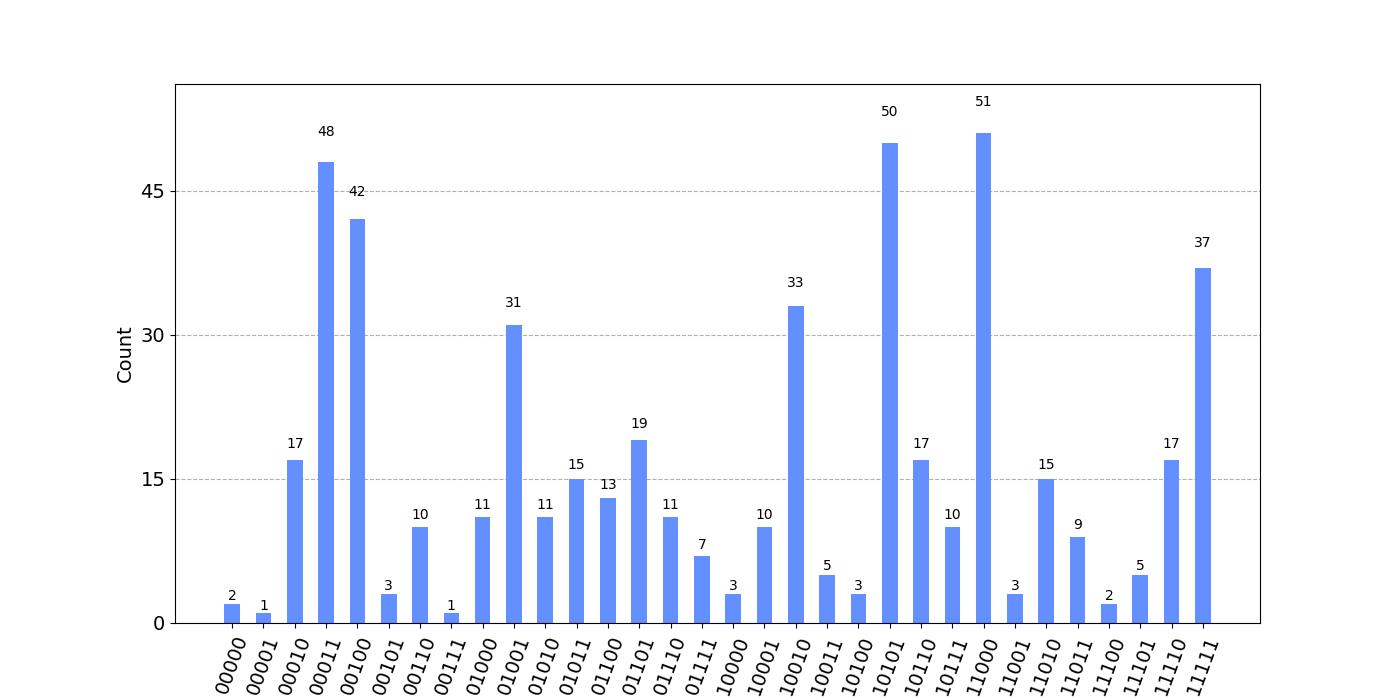
\includegraphics[scale=0.4]{./img/primer_grafo/sin_restriccion_extra/primer_provider_iter-2.png}
\caption{num iterations=2}
\end{figure}

\newpage

\subsubsection{ibmq\textunderscore manila}
\label{sec:orgc2b07c5}
\(\beta\)\textsubscript{0} = 0.5, \(\gamma\)\textsubscript{0} = 0.5
\begin{center}
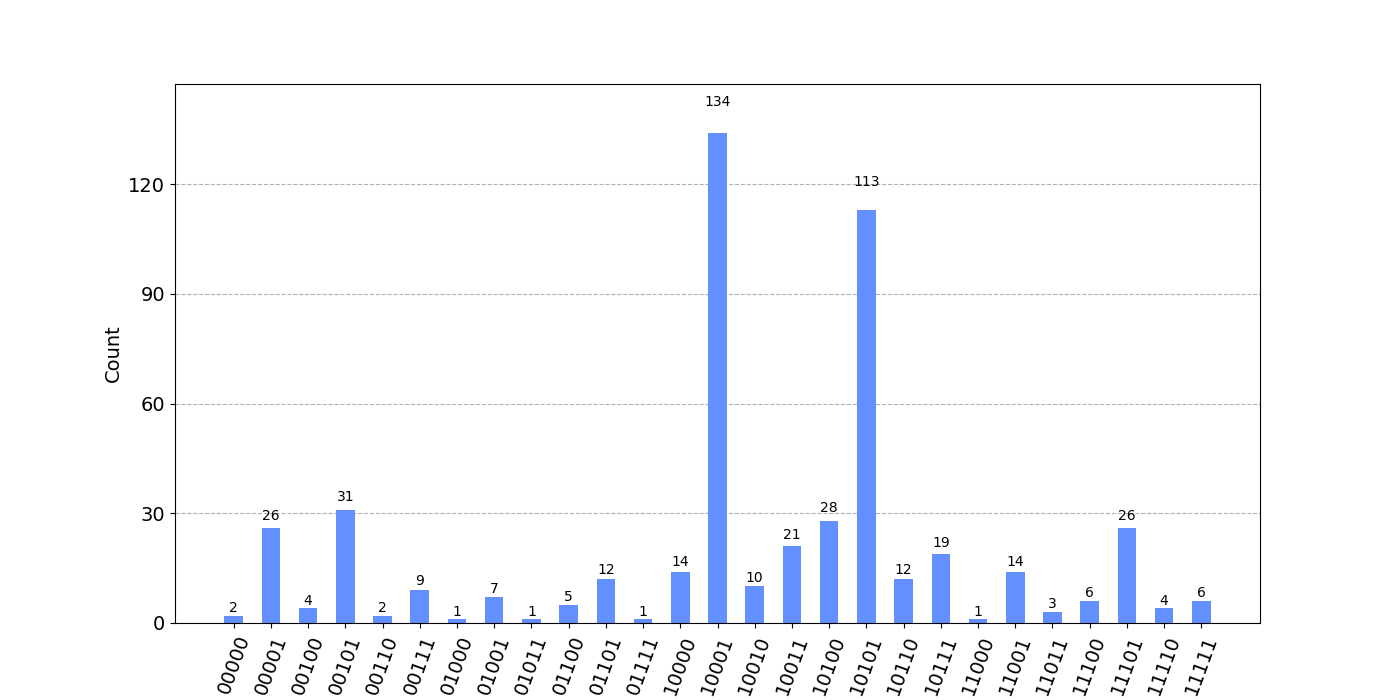
\includegraphics[scale=0.4]{./img/primer_grafo/sin_restriccion_extra/primer_provider_manila.png}
\end{center}
\newpage

\subsection{Runtime}
\label{sec:orgbceff6b}
\subsubsection{ibmq\textunderscore lima}
\label{sec:orgd98e5ef}
\(\beta\)\textsubscript{0} = 0.5, \(\gamma\)\textsubscript{0} = 0.5
\begin{center}
\begin{tabular}{|r|l|r|}
\hline
\textbf{fun} & \textbf{theta} & \textbf{num iterations}\\
\hline
37.16 & [0.6869, 0.4728] & 26\\
\hline
\end{tabular}
\end{center}


Resultado de ejecutar ese \textbf{theta} obtenido con Aer:
\begin{center}
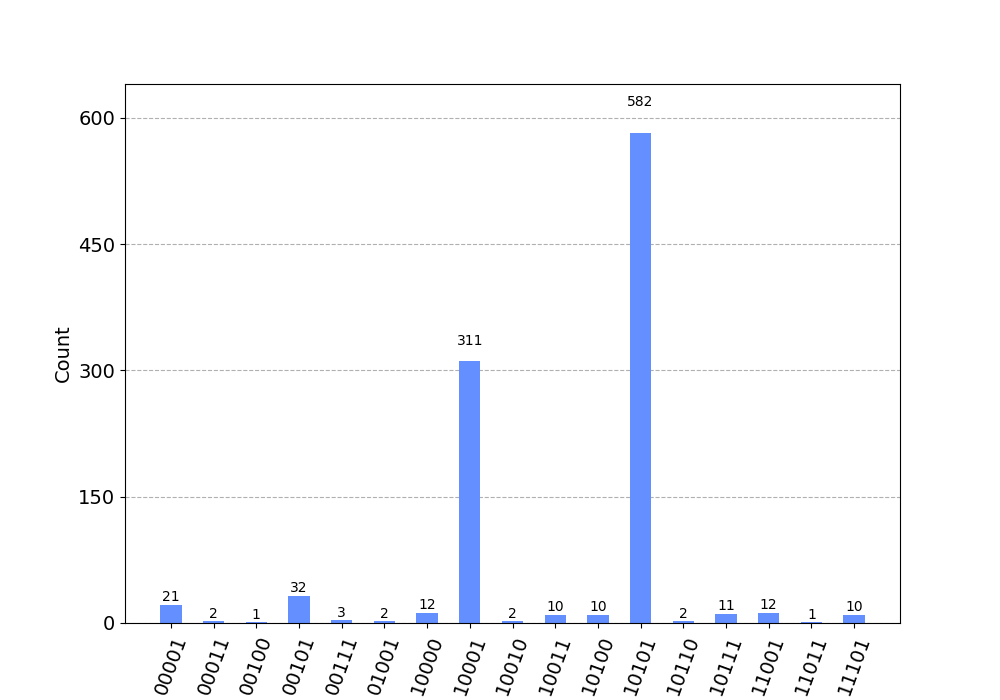
\includegraphics[scale=0.4]{./img/primer_grafo/sin_restriccion_extra/primer_runtime_lima.png}
\end{center}

\newpage
\section{Primer grafo con restricción}
\label{sec:org68585df}
\subsection{Aer simulator con restricción extra  (primer\textunderscore grafo/con\textunderscore restricc/aer-qaoa.ipynb)}
\label{sec:org8f3ae61}
Con respecto a la función de coste del paper se añade la restricción\newline
    \textbf{X\textsubscript{13} + X\textsubscript{23} = 1}\newline
Esto sería, que el camino solo llegue al nodo final \textbf{3} por una de las aristas X\textsubscript{i3} existentes.

\uline{Modificadores del paper}

\begin{itemize}
\item Estadísticas num layers = 1:
\end{itemize}
\begin{center}
\begin{tabular}{|r|l|r|}
\hline
\textbf{Qubits} & \textbf{Camino} & \textbf{Frecuencia (1000)}\\
\hline
10101 & \textbf{Óptimo} & 938\\
11000 &  & 37\\
10001 &  & 9\\
00011 &  & 11\\
00100 &  & 3\\
00010 &  & 1\\
11111 &  & 1\\
\hline
\end{tabular}
\end{center}

\begin{itemize}
\item Estadísticas num layers = 2:
\end{itemize}
\begin{center}
\begin{tabular}{|r|l|r|}
\hline
\textbf{Qubits} & \textbf{Camino} & \textbf{Frecuencia (1000)}\\
\hline
10101 & \textbf{Óptimo} & 646\\
01010 &  & 159\\
10001 &  & 58\\
01001 &  & 42\\
10010 &  & 28\\
00100 &  & 19\\
11011 &  & 18\\
\ldots{} &  & \ldots{}\\
\hline
\end{tabular}
\end{center}

\begin{itemize}
\item Estadísticas num layers = 3:
\end{itemize}
\begin{center}
\begin{tabular}{|r|l|r|}
\hline
\textbf{Qubits} & \textbf{Camino} & \textbf{Frecuencia (1000)}\\
\hline
10101 & \textbf{Óptimo} & 848\\
10001 &  & 67\\
10010 &  & 25\\
01001 &  & 16\\
01010 &  & 10\\
10110 &  & 6\\
11101 &  & 4\\
\ldots{} &  & \ldots{}\\
\hline
\end{tabular}
\end{center}

\newpage

\subsubsection{Caso correcto num layers = 1}
\label{sec:org4131c74}
\begin{center}
\begin{tabular}{|r|l|r|r|}
\hline
\textbf{fun} & \textbf{theta} & \textbf{num iterations} & \textbf{seed\textunderscore simulator}\\
\hline
42.29 & [0.5081, 0.9401] & 33 & 3\\
\hline
\end{tabular}
\end{center}

\begin{figure}[htbp]
\centering
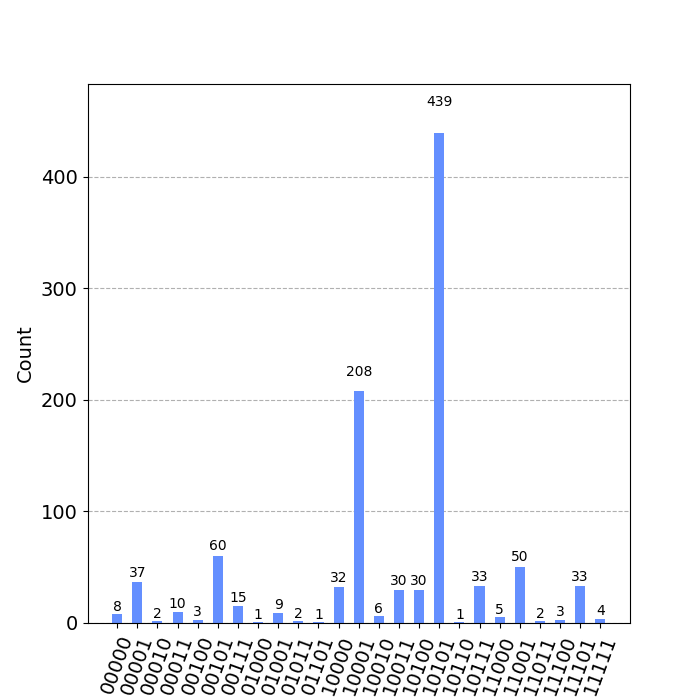
\includegraphics[scale=0.5]{./img/primer_grafo/con_restriccion_extra/primer_restr_aer_correcto.png}
\caption{seed\textunderscore simulator=3}
\end{figure}

Mejor resultado: 10101 (q\textsubscript{4}q\textsubscript{3}q\textsubscript{2}q\textsubscript{1}q\textsubscript{0} = X\textsubscript{23}X\textsubscript{13}X\textsubscript{12}X\textsubscript{02}X\textsubscript{01})

Camino: X\textsubscript{01}X\textsubscript{12}X\textsubscript{23} (Camino óptimo)

\newpage

\subsubsection{Caso "correcto" con ruido num layers = 1}
\label{sec:orgaf841c6}
\begin{table}[htbp]
\caption{captionada}
\centering
\begin{tabular}{|r|l|r|r|}
\hline
\textbf{fun} & \textbf{theta} & \textbf{num iterations} & \textbf{seed\textunderscore simulator}\\
\hline
90.75 & [0.9962, 1.995] & 27 & 2\\
\hline
\end{tabular}
\end{table}

\begin{figure}[htbp]
\centering
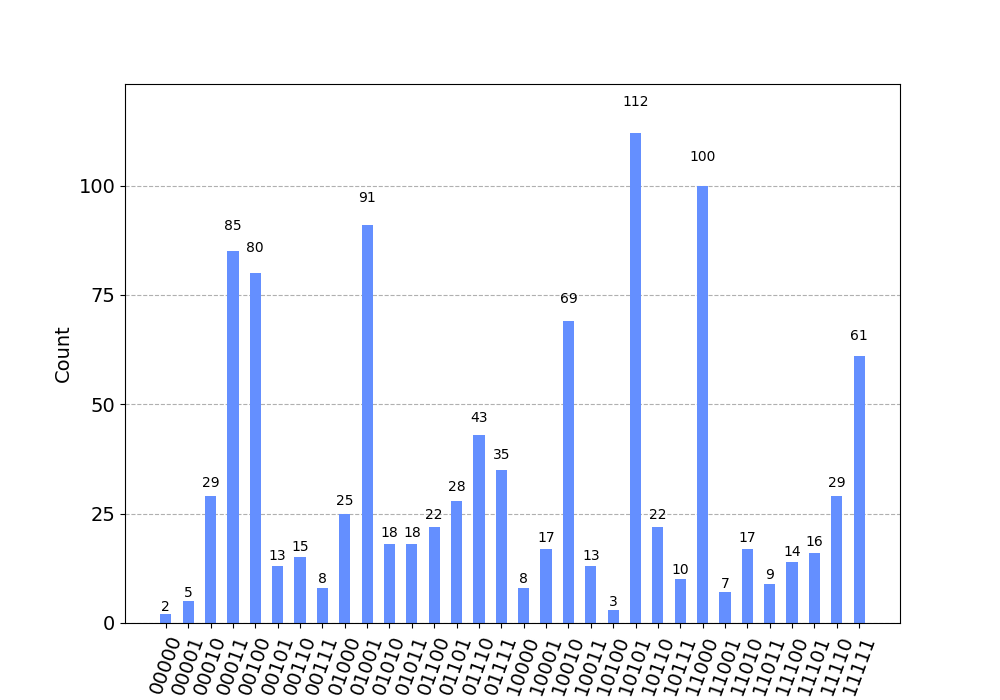
\includegraphics[scale=0.5]{./img/primer_grafo/con_restriccion_extra/primer_restr_aer_correcto-con-ruido.png}
\caption{seed\textunderscore simulator=2}
\end{figure}

Mejor resultado: 10101 (q\textsubscript{4}q\textsubscript{3}q\textsubscript{2}q\textsubscript{1}q\textsubscript{0} = X\textsubscript{23}X\textsubscript{13}X\textsubscript{12}X\textsubscript{02}X\textsubscript{01})

Camino: X\textsubscript{01}X\textsubscript{12}X\textsubscript{23} (Camino óptimo)

Aunque se obtenga el resultado óptimo (10101) existen otros resultados demasiado altos, e incluso ejecutando el circuito con el mismo \textbf{theta} se dan valores distintos. Podría afectar a los resultados de las estadísticas.

Además se ve que encuentra un valor \textbf{fun} demasiado alto (90.75)

\newpage

\subsubsection{Gamma function}
\label{sec:org0fe23cf}
Variación de execute\textunderscore circuit con respecto a \(\gamma\) con num layers = 1 y \(\beta\) = 1.0
\begin{center}
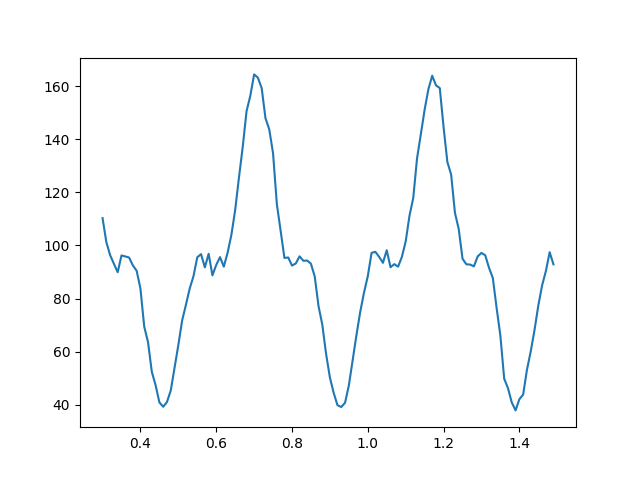
\includegraphics[width=.9\linewidth]{./img/primer_grafo/con_restriccion_extra/primer_restr_aer_gamma_fun.png}
\end{center}

\subsection{Aer simulator con restricción extra y P = 40}
\label{sec:org620e228}
\subsubsection{Modificadores del paper}
\label{sec:org1e3aafd}
\lstset{language=Python,label= ,caption= ,captionpos=b,numbers=none}
\begin{lstlisting}
circuit.rz(coef, q_idx)
circuit.rzz(coef * gamma[p], q_idxs[0], q_idxs[1])
circuit.rx(beta[p] * 2, q_idx)
\end{lstlisting}

\begin{itemize}
\item Estadísticas num layers = 1:
\begin{center}
\begin{tabular}{|r|l|r|}
\hline
\textbf{Qubits} & \textbf{Camino} & \textbf{Frecuencia (1000)}\\
\hline
10001 &  & 825\\
10101 & \textbf{Óptimo} & 174\\
01010 &  & 1\\
\hline
\end{tabular}
\end{center}

\item Estadísticas num layers = 2:
\begin{center}
\begin{tabular}{|r|l|r|}
\hline
\textbf{Qubits} & \textbf{Camino} & \textbf{Frecuencia (1000)}\\
\hline
10101 & \textbf{Óptimo} & 544\\
10001 &  & 152\\
01010 &  & 94\\
01001 &  & 84\\
10010 &  & 62\\
11001 &  & 27\\
10110 &  & 15\\
\ldots{} &  & \ldots{}\\
\hline
\end{tabular}
\end{center}

\item Estadísticas num layers = 3:
\begin{center}
\begin{tabular}{|r|l|r|}
\hline
\textbf{Qubits} & \textbf{Camino} & \textbf{Frecuencia (1000)}\\
\hline
10101 & \textbf{Óptimo} & 693\\
01001 &  & 69\\
10001 &  & 65\\
10010 &  & 42\\
01010 &  & 31\\
00011 &  & 26\\
01011 &  & 20\\
11001 &  & 14\\
00010 &  & 10\\
\ldots{} &  & \ldots{}\\
\hline
\end{tabular}
\end{center}
\end{itemize}
\newpage

\subsubsection{Modificadores originales}
\label{sec:org79ffdbb}
\lstset{language=Python,label= ,caption= ,captionpos=b,numbers=none}
\begin{lstlisting}
circuit.rz(coef * gamma[p] * 2, q_idx)
circuit.rzz(coef * gamma[p] * 2, q_idxs[0], q_idxs[1])
circuit.rx(beta[p] * 2, q_idx)
\end{lstlisting}

\begin{itemize}
\item Estadísticas num layers = 1:
\begin{center}
\begin{tabular}{|r|l|r|}
\hline
\textbf{Qubits} & \textbf{Camino} & \textbf{Frecuencia (1000)}\\
\hline
10101 & \textbf{Óptimo} & 630\\
00001 &  & 139\\
11001 &  & 99\\
10001 &  & 39\\
10011 &  & 36\\
01001 &  & 28\\
10010 &  & 14\\
\ldots{} &  & \ldots{}\\
\hline
\end{tabular}
\end{center}

\item Estadísticas num layers = 2:
\begin{center}
\begin{tabular}{|r|l|r|}
\hline
\textbf{Qubits} & \textbf{Camino} & \textbf{Frecuencia (1000)}\\
\hline
10101 & \textbf{Óptimo} & 382\\
10001 &  & 167\\
01001 &  & 105\\
10010 &  & 73\\
00000 &  & 43\\
\ldots{} &  & \ldots{}\\
\hline
\end{tabular}
\end{center}

\item Estadísticas num layers = 3:
\begin{center}
\begin{tabular}{|r|l|r|}
\hline
\textbf{Qubits} & \textbf{Camino} & \textbf{Frecuencia (1000)}\\
\hline
10101 & \textbf{Óptimo} & 412\\
01001 &  & 134\\
10010 &  & 93\\
10001 &  & 83\\
00001 &  & 81\\
\ldots{} &  & \ldots{}\\
\hline
\end{tabular}
\end{center}
\end{itemize}

\subsubsection{Conclusiones y Gamma function}
\label{sec:org355de8b}
\begin{itemize}
\item Para ambos modificadores los resultados sí parecen mejorar con el número de capas (aunque den resultados muy bajos)
\end{itemize}
\begin{enumerate}
\item Modificadores del paper
\label{sec:org602ba0e}
\begin{center}
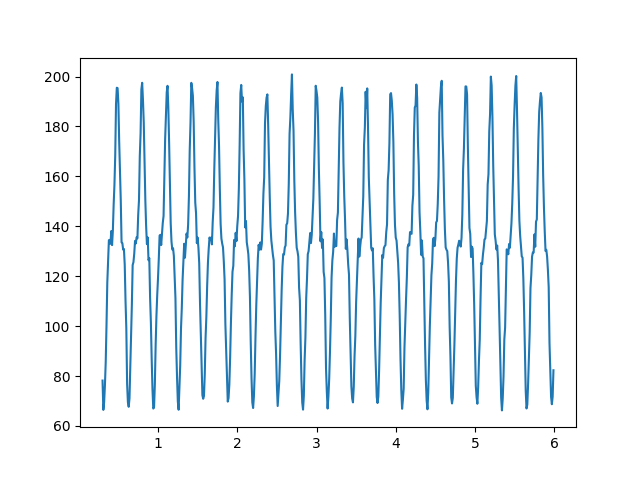
\includegraphics[width=.9\linewidth]{./img/primer_grafo/con_restriccion_extra/primer_p_40_mod-paper_gamma_fun.png}
\end{center}
\item Modificadores originales
\label{sec:org03aef46}
\begin{center}
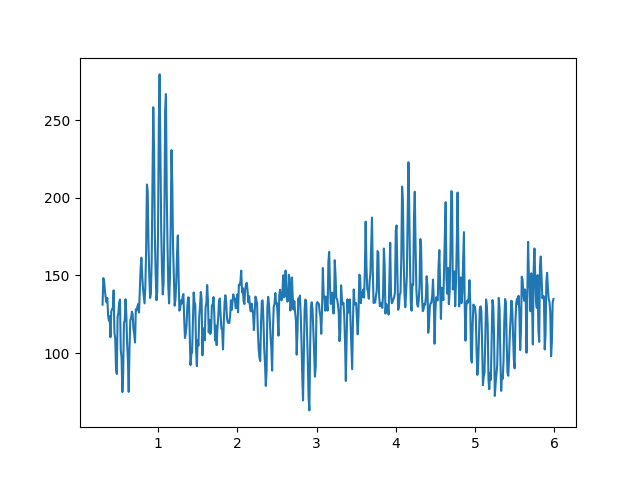
\includegraphics[width=.9\linewidth]{./img/primer_grafo/con_restriccion_extra/primer_p_40_mod-originales_gamma_fun.png}
\end{center}
\newpage
\end{enumerate}
\subsection{Aer simulator con restricción extra y P = 54}
\label{sec:org562bbaa}
\lstset{language=Python,label= ,caption= ,captionpos=b,numbers=none}
\begin{lstlisting}
circuit.rz(coef, q_idx)
circuit.rzz(coef * gamma[p], q_idxs[0], q_idxs[1])
circuit.rx(beta[p] * 2, q_idx)
\end{lstlisting}
Probar a aumentar el factor de penalización para las restricciones (P = 54).
\begin{itemize}
\item Estadísticas num layers = 1:
\begin{center}
\begin{tabular}{|r|l|r|}
\hline
\textbf{Qubits} & \textbf{Camino} & \textbf{Frecuencia (1000)}\\
\hline
10010 &  & 251\\
01010 &  & 236\\
01001 &  & 222\\
10101 & \textbf{Óptimo} & 135\\
10001 &  & 100\\
00001 &  & 46\\
01101 &  & 4\\
10110 &  & 3\\
00101 &  & 1\\
00000 &  & 1\\
10111 &  & 1\\
\hline
\end{tabular}
\end{center}

\begin{itemize}
\item Estadísticas num layers = 2:
\end{itemize}
\begin{center}
\begin{tabular}{|r|l|r|}
\hline
\textbf{Qubits} & \textbf{Camino} & \textbf{Frecuencia (1000)}\\
\hline
01010 &  & 280\\
10010 &  & 199\\
01001 &  & 190\\
10101 & \textbf{Óptimo} & 183\\
10001 &  & 85\\
00001 &  & 37\\
01101 &  & 13\\
10110 &  & 7\\
11010 &  & 2\\
00000 &  & 2\\
11011 &  & 1\\
00010 &  & 1\\
\hline
\end{tabular}
\end{center}
\end{itemize}
\newpage

\subsubsection{Gamma function}
\label{sec:org33b0248}
Variación de execute\textunderscore circuit con respecto a \(\gamma\) con num layers = 1 y \(\beta\) = 1.0
\begin{center}
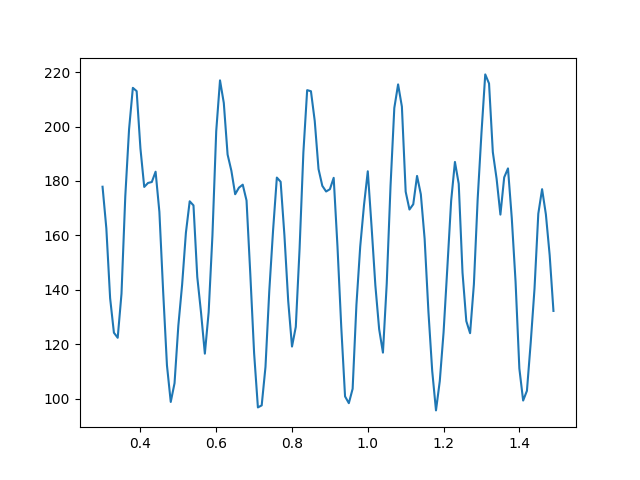
\includegraphics[width=.9\linewidth]{./img/primer_grafo/con_restriccion_extra/primer_p_54_gamma_fun.png}
\end{center}

\newpage

\section{Grafo Zhiqiang (Con aer)}
\label{sec:orgae63ca4}
\begin{center}
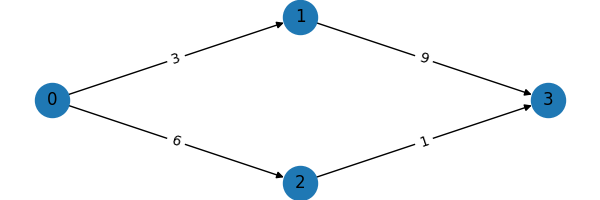
\includegraphics[width=.9\linewidth]{./img/zhiqiang_grafo/zhiqiang_grafo.png}
\end{center}
\subsection{Modificadores originales}
\label{sec:org46a75f7}
\lstset{language=Python,label= ,caption= ,captionpos=b,numbers=none}
\begin{lstlisting}
circuit.rz(coef * gamma[p] * 2, q_idx)
circuit.rzz(coef * gamma[p] * 2, q_idxs[0], q_idxs[1])
circuit.rx(beta[p] * 2, q_idx)
\end{lstlisting}

\subsubsection{P=20}
\label{sec:orgf5d0f9a}

\begin{itemize}
\item Estadísticas num layers = 1:
\begin{center}
\begin{tabular}{|r|l|r|}
\hline
\textbf{Qubits} & \textbf{Camino} & \textbf{Frecuencia} (1000)\\
\hline
0101 & X\textsubscript{01}X\textsubscript{13} & 912\\
0110 &  & 86\\
1010 & X\textsubscript{02}X\textsubscript{23} -> Óptimo & 1\\
0111 &  & 1\\
\hline
\end{tabular}
\end{center}

\item Estadísticas num layers = 2:
\begin{center}
\begin{tabular}{|r|l|r|}
\hline
\textbf{Qubits} & \textbf{Camino} & \textbf{Frecuencia} (1000)\\
\hline
0101 &  & 965\\
0000 &  & 22\\
1010 & \textbf{Óptimo} & 8\\
0001 &  & 2\\
1001 &  & 1\\
0110 &  & 1\\
1000 &  & 1\\
\hline
\end{tabular}
\end{center}

\item Estadísticas num layers = 4:
\begin{center}
\begin{tabular}{|r|l|r|}
\hline
\textbf{Qubits} & \textbf{Camino} & \textbf{Frecuencia} (1000)\\
\hline
0101 &  & 985\\
1010 & \textbf{Óptimo} & 15\\
\hline
\end{tabular}
\end{center}

\item Estadísticas num layers = 10:
\begin{center}
\begin{tabular}{|r|l|r|}
\hline
\textbf{Qubits} & \textbf{Camino} & \textbf{Frecuencia} (1000)\\
\hline
1010 & \textbf{Óptimo} & 687\\
0101 &  & 308\\
0000 &  & 2\\
0001 &  & 1\\
0100 &  & 1\\
1110 &  & 1\\
\hline
\end{tabular}
\end{center}
\end{itemize}

\begin{enumerate}
\item Gamma function
\label{sec:org37e91f3}

Variación de execute\textunderscore circuit con respecto a \(\gamma\) con num layers = 1 y \(\beta\) = 1.0
\begin{center}
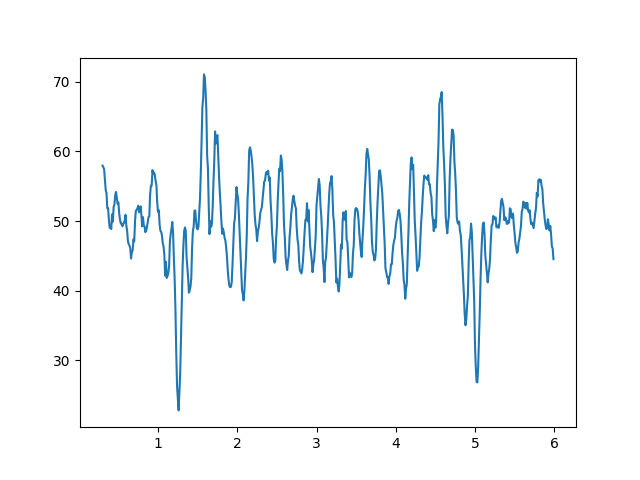
\includegraphics[width=.9\linewidth]{./img/zhiqiang_grafo/modificadores_originales/zhiqiang_p_20_gamma_fun.png}
\end{center}

\newpage
\end{enumerate}

\subsubsection{P=40}
\label{sec:org82096cc}

\begin{itemize}
\item Estadísticas num layers = 1:
\begin{center}
\begin{tabular}{|r|l|r|}
\hline
\textbf{Qubits} & \textbf{Camino} & \textbf{Frecuencia} (1000)\\
\hline
1000 &  & 260\\
1010 & \textbf{Óptimo} & 202\\
1001 &  & 147\\
0101 &  & 141\\
1101 &  & 66\\
1011 &  & 59\\
1111 &  & 29\\
0001 &  & 23\\
0100 &  & 20\\
0010 &  & 17\\
0000 &  & 13\\
0110 &  & 12\\
0111 &  & 7\\
1110 &  & 4\\
\hline
\end{tabular}
\end{center}

\item Estadísticas num layers = 2:
\begin{center}
\begin{tabular}{|r|l|r|}
\hline
\textbf{Qubits} & \textbf{Camino} & \textbf{Frecuencia} (1000)\\
\hline
1010 & \textbf{Óptimo} & 481\\
0101 &  & 215\\
1001 &  & 62\\
0000 &  & 55\\
0010 &  & 50\\
1000 &  & 31\\
0100 &  & 26\\
1101 &  & 22\\
1011 &  & 17\\
1110 &  & 16\\
0001 &  & 8\\
0110 &  & 6\\
0111 &  & 6\\
1111 &  & 5\\
\hline
\end{tabular}
\end{center}

\item Estadísticas num layers = 3:
\begin{center}
\begin{tabular}{|r|l|r|}
\hline
\textbf{Qubits} & \textbf{Camino} & \textbf{Frecuencia} (1000)\\
\hline
1010 & \textbf{Óptimo} & 513\\
0101 &  & 387\\
1000 &  & 33\\
1101 &  & 21\\
1001 &  & 21\\
1110 &  & 6\\
0000 &  & 5\\
1111 &  & 4\\
1011 &  & 4\\
0111 &  & 3\\
0010 &  & 2\\
0100 &  & 1\\
\hline
\end{tabular}
\end{center}

\item Estadísticas num layers = 10:
\begin{center}
\begin{tabular}{|r|l|r|}
\hline
\textbf{Qubits} & \textbf{Camino} & \textbf{Frecuencia} (1000)\\
\hline
1010 & \textbf{Óptimo} & 564\\
0101 &  & 431\\
0100 &  & 2\\
0111 &  & 1\\
1110 &  & 1\\
0000 &  & 1\\
\hline
\end{tabular}
\end{center}
\end{itemize}

\begin{enumerate}
\item Gamma function
\label{sec:orgba03a16}

Variación de execute\textunderscore circuit con respecto a \(\gamma\) con num layers = 1 y \(\beta\) = 1.0
\begin{center}
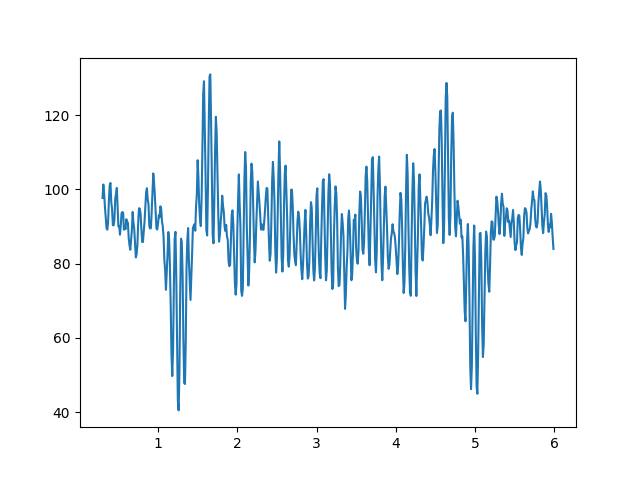
\includegraphics[width=.9\linewidth]{./img/zhiqiang_grafo/modificadores_originales/zhiqiang_p_40_gamma_fun.png}
\end{center}
\newpage
\end{enumerate}

\subsubsection{Conclusiones}
\label{sec:orgfc72854}
\begin{itemize}
\item A diferencia de "primer grafo" con P=20 los resultados mejoran al aumentar el número de capas, aunque siguen siendo muy malos resultados.
\item Los resultados de la función con respecto a \(\gamma\) son muy ruidosos, puede ser el motivo de tan malos resultados.
\item Al utilizar P=40 se obtiene una gráfica más ruidosa y con valores mucho más altos al romper restricciones. Esto es de esperar, ya que P se utiliza como factor de penalización en la función de coste (P*(\ldots{})\textsuperscript{2}).
\item El aumento de P puede estar provocando que resultados de función cercanos al óptimo sean menos probables (en las gráficas con P=20 hay un mínimo \textasciitilde{}= 20 y con P=20 es \textasciitilde{}= 40)
\end{itemize}

\newpage

\subsection{Modificadores del paper}
\label{sec:org453c51b}
\lstset{language=Python,label= ,caption= ,captionpos=b,numbers=none}
\begin{lstlisting}
circuit.rz(coef, q_idx)
circuit.rzz(coef * gamma[p], q_idxs[0], q_idxs[1])
circuit.rx(beta[p] * 2, q_idx)
\end{lstlisting}

\subsubsection{P=20}
\label{sec:orgb34a8a6}
\begin{itemize}
\item Estadísticas num layers = 1:
\begin{center}
\begin{tabular}{|r|l|r|}
\hline
\textbf{Qubits} & \textbf{Camino} & \textbf{Frecuencia} (1000)\\
\hline
1101 &  & 381\\
1001 &  & 182\\
0010 &  & 178\\
1011 &  & 97\\
0110 &  & 44\\
0100 &  & 44\\
0001 &  & 26\\
\ldots{} &  & \ldots{}\\
1010 & \textbf{Óptimo} & 4\\
\ldots{} &  & \ldots{}\\
\hline
\end{tabular}
\end{center}

\item Estadísticas num layers = 2:
\begin{center}
\begin{tabular}{|r|l|r|}
\hline
\textbf{Qubits} & \textbf{Camino} & \textbf{Frecuencia} (1000)\\
\hline
1010 & \textbf{Óptimo} & 324\\
0101 &  & 285\\
1011 &  & 268\\
1001 &  & 102\\
1110 &  & 20\\
0100 &  & 1\\
\hline
\end{tabular}
\end{center}

\item Estadísticas num layers = 3:
\begin{center}
\begin{tabular}{|r|l|r|}
\hline
\textbf{Qubits} & \textbf{Camino} & \textbf{Frecuencia} (1000)\\
\hline
1010 & \textbf{Óptimo} & 928\\
0101 &  & 68\\
1011 &  & 4\\
\hline
\end{tabular}
\end{center}
\end{itemize}

\newpage
\begin{enumerate}
\item Gamma function
\label{sec:org93d6f09}

Variación de execute\textunderscore circuit con respecto a \(\gamma\) con num layers = 1 y \(\beta\) = 1.0
\begin{center}
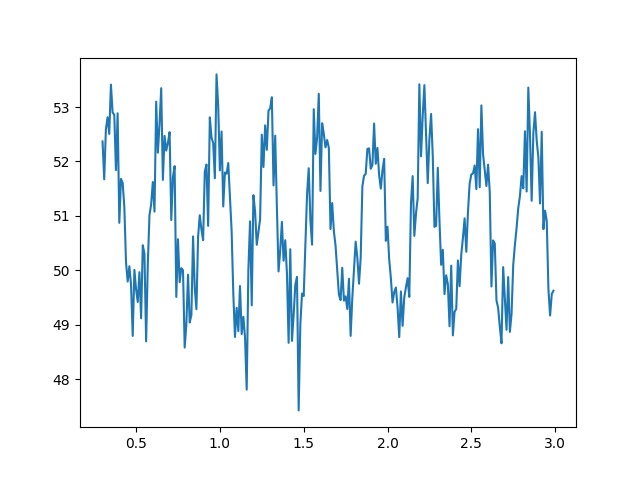
\includegraphics[width=.9\linewidth]{./img/zhiqiang_grafo/modificadores_paper/zhiqiang_p_20_gamma_fun.png}
\end{center}
\newpage
\end{enumerate}

\subsubsection{P=40}
\label{sec:org04d9aa9}
\begin{itemize}
\item Estadísticas num layers = 1:
\begin{center}
\begin{tabular}{|r|l|r|}
\hline
\textbf{Qubits} & \textbf{Camino} & \textbf{Frecuencia} (1000)\\
\hline
1101 &  & 714\\
0100 &  & 124\\
0010 &  & 47\\
0110 &  & 85\\
1000 &  & 2\\
1001 &  & 11\\
1011 &  & 10\\
1110 &  & 2\\
0111 &  & 1\\
1111 &  & 1\\
0001 &  & 2\\
0000 &  & 1\\
\hline
\end{tabular}
\end{center}
\end{itemize}
El óptimo ni siquiera aparece (\textbf{0\%})

\begin{itemize}
\item Estadísticas num layers = 2:
\begin{center}
\begin{tabular}{|r|l|r|}
\hline
\textbf{Qubits} & \textbf{Camino} & \textbf{Frecuencia} (1000)\\
\hline
1010 & \textbf{Óptimo} & 392\\
0100 &  & 182\\
0110 &  & 148\\
0010 &  & 139\\
\ldots{} &  & \ldots{}\\
\hline
\end{tabular}
\end{center}

\item Estadísticas num layers = 3:
\begin{center}
\begin{tabular}{|r|l|r|}
\hline
\textbf{Qubits} & \textbf{Camino} & \textbf{Frecuencia} (1000)\\
\hline
1010 & \textbf{Óptimo} & 637\\
0101 &  & 183\\
1101 &  & 71\\
1011 &  & 42\\
0100 &  & 18\\
0110 &  & 13\\
1001 &  & 11\\
1110 &  & 9\\
0010 &  & 7\\
0000 &  & 4\\
0001 &  & 3\\
1000 &  & 2\\
\hline
\end{tabular}
\end{center}

\item Estadísticas num layers = 4:
\begin{center}
\begin{tabular}{|r|l|r|}
\hline
\textbf{Qubits} & \textbf{Camino} & \textbf{Frecuencia} (1000)\\
\hline
0101 &  & 661\\
1010 & \textbf{Óptimo} & 337\\
0100 &  & 1\\
1101 &  & 1\\
\hline
\end{tabular}
\end{center}

\item Estadísticas num layers = 10:
\begin{center}
\begin{tabular}{|r|l|r|}
\hline
\textbf{Qubits} & \textbf{Camino} & \textbf{Frecuencia} (1000)\\
\hline
0101 &  & 568\\
1010 & \textbf{Óptimo} & 426\\
1000 &  & 1\\
0111 &  & 1\\
0010 &  & 1\\
0000 &  & 2\\
1101 &  & 1\\
\hline
\end{tabular}
\end{center}
\end{itemize}

\begin{enumerate}
\item Gamma function
\label{sec:org67fd110}

Variación de execute\textunderscore circuit con respecto a \(\gamma\) con num layers = 1 y \(\beta\) = 1.0
\begin{center}
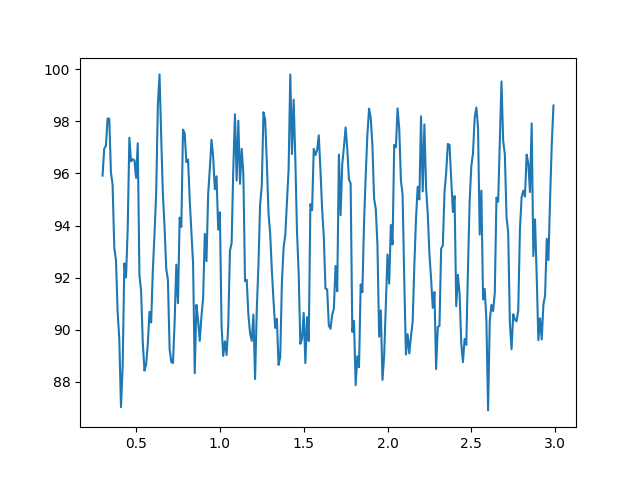
\includegraphics[width=.9\linewidth]{./img/zhiqiang_grafo/modificadores_paper/zhiqiang_p_40_gamma_fun.png}
\end{center}
\newpage
\end{enumerate}

\subsubsection{Conclusiones}
\label{sec:orgbc2a77c}
\begin{itemize}
\item Mejora muy clara con el aumento de capas (con P=20 y 3 capas se acierta un \textbf{92.8\%}).
\end{itemize}

\newpage
\section{DWave}
\label{sec:orgd7e336e}
Ejecuciones con 1024 medidas
\subsection{Primer grafo}
\label{sec:org36476b8}
\begin{center}
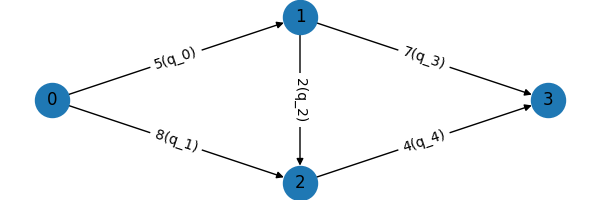
\includegraphics[width=.9\linewidth]{./img/primer_grafo/primer_grafo.png}
\end{center}

Sampleset:
\begin{center}
\begin{tabular}{|r|r|r|r|r|r|r|r|r|}
\hline
 & (0, 1) & (0, 2) & (1, 2) & (1, 3) & (2, 3) & energy & num oc. & chain .\\
\hline
0 & 1 & 0 & 1 & 0 & 1 & 11.0 & 348 & 0.0\\
1 & 0 & 1 & 0 & 0 & 1 & 12.0 & 373 & 0.0\\
2 & 1 & 0 & 0 & 1 & 0 & 12.0 & 294 & 0.0\\
3 & 0 & 0 & 0 & 0 & 0 & 54.0 & 4 & 0.0\\
4 & 0 & 0 & 0 & 0 & 1 & 58.0 & 1 & 0.0\\
5 & 1 & 0 & 0 & 0 & 0 & 59.0 & 1 & 0.0\\
6 & 0 & 0 & 1 & 0 & 1 & 60.0 & 1 & 0.0\\
7 & 1 & 0 & 1 & 0 & 0 & 61.0 & 1 & 0.0\\
8 & 0 & 1 & 0 & 1 & 0 & 69.0 & 1 & 0.0\\
\hline
\end{tabular}
\end{center}
['BINARY', 9 rows, 1024 samples, 5 variables]

\newpage
\subsection{Segundo grafo}
\label{sec:org8bae427}
\begin{center}
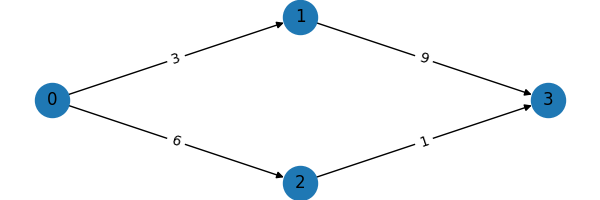
\includegraphics[width=.9\linewidth]{./img/segundo_grafo.png}
\end{center}

Sampleset:
\begin{center}
\begin{tabular}{|r|r|r|r|r|r|r|l|r|r|r|l|}
\hline
 & (0, 1) & (0, 2) & (0, 3) & (1, 2) & (1, 3) & (2, 3) & \ldots{} & (4, 5) & energy & num oc. & \ldots{}\\
\hline
0 & 0 & 1 & 0 & 0 & 0 & 0 & \ldots{} & 1 & 4.0 & 72 & \ldots{}\\
1 & 0 & 1 & 0 & 0 & 0 & 0 & \ldots{} & 1 & 6.0 & 69 & \ldots{}\\
2 & 0 & 1 & 0 & 0 & 0 & 1 & \ldots{} & 1 & 7.0 & 65 & \ldots{}\\
3 & 1 & 0 & 0 & 1 & 0 & 0 & \ldots{} & 1 & 7.0 & 37 & \ldots{}\\
134 & 0 & 1 & 0 & 0 & 0 & 1 & \ldots{} & 1 & 7.0 & 1 & \ldots{}\\
4 & 0 & 0 & 1 & 0 & 0 & 0 & \ldots{} & 1 & 8.0 & 51 & \ldots{}\\
5 & 0 & 1 & 0 & 0 & 0 & 0 & \ldots{} & 0 & 8.0 & 92 & \ldots{}\\
6 & 1 & 0 & 0 & 0 & 1 & 0 & \ldots{} & 1 & 8.0 & 42 & \ldots{}\\
7 & 0 & 1 & 0 & 0 & 0 & 1 & \ldots{} & 0 & 9.0 & 47 & \ldots{}\\
8 & 1 & 0 & 0 & 1 & 0 & 0 & \ldots{} & 1 & 9.0 & 34 & \ldots{}\\
9 & 1 & 0 & 0 & 0 & 1 & 0 & \ldots{} & 0 & 10.0 & 29 & \ldots{}\\
10 & 1 & 0 & 0 & 1 & 0 & 1 & \ldots{} & 1 & 10.0 & 33 & \ldots{}\\
11 & 0 & 0 & 1 & 0 & 0 & 0 & \ldots{} & 0 & 10.0 & 39 & \ldots{}\\
12 & 0 & 1 & 0 & 0 & 0 & 1 & \ldots{} & 0 & 11.0 & 53 & \ldots{}\\
13 & 1 & 0 & 0 & 1 & 0 & 0 & \ldots{} & 0 & 11.0 & 29 & \ldots{}\\
14 & 1 & 0 & 0 & 0 & 1 & 0 & \ldots{} & 0 & 12.0 & 35 & \ldots{}\\
15 & 1 & 0 & 0 & 1 & 0 & 1 & \ldots{} & 0 & 12.0 & 32 & \ldots{}\\
16 & 0 & 0 & 1 & 0 & 0 & 0 & \ldots{} & 0 & 12.0 & 54 & \ldots{}\\
17 & 1 & 0 & 0 & 1 & 0 & 1 & \ldots{} & 0 & 14.0 & 42 & \ldots{}\\
20 & 0 & 1 & 0 & 0 & 0 & 0 & \ldots{} & 0 & 55.0 & 3 & \ldots{}\\
\ldots{} & \ldots{} & \ldots{} & \ldots{} & \ldots{} & \ldots{} & \ldots{} & \ldots{} & \ldots{} & \ldots{} & \ldots{} & \ldots{}\\
\hline
\end{tabular}
\end{center}
['BINARY', 137 rows, 1024 samples, 11 variables]

\newpage
\subsection{Zhiqiang grafo}
\label{sec:org7f5ddfe}
\begin{center}
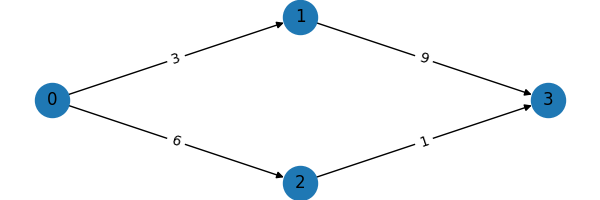
\includegraphics[width=.9\linewidth]{./img/zhiqiang_grafo/zhiqiang_grafo.png}
\end{center}

Sampleset:
\begin{center}
\begin{tabular}{|r|r|r|r|r|r|r|r|}
\hline
 & (0, 1) & (0, 2) & (1, 3) & (2, 3) & energy & num oc. & chain .\\
\hline
0 & 0 & 1 & 0 & 1 & 7.0 & 776 & 0.0\\
1 & 1 & 0 & 1 & 0 & 12.0 & 247 & 0.0\\
2 & 0 & 1 & 0 & 0 & 46.0 & 1 & 0.0\\
\hline
\end{tabular}
\end{center}
\end{document}